% Created 2022-06-21 Tue 15:13
% Intended LaTeX compiler: pdflatex
\documentclass[11pt]{article}
\usepackage[utf8]{inputenc}
\usepackage[T1]{fontenc}
\usepackage{graphicx}
\usepackage{longtable}
\usepackage{wrapfig}
\usepackage{rotating}
\usepackage[normalem]{ulem}
\usepackage{amsmath}
\usepackage{amssymb}
\usepackage{capt-of}
\usepackage{hyperref}
\hypersetup{colorlinks=true,linkcolor=grey}
\hypersetup{colorlinks=true,linkcolor=grey}
\author{Y. Sahli}
\date{\today}
\title{UE4: Dispensation des Médicaments et Autres Produits de Santé}
\hypersetup{
 pdfauthor={Y. Sahli},
 pdftitle={UE4: Dispensation des Médicaments et Autres Produits de Santé},
 pdfkeywords={},
 pdfsubject={},
 pdfcreator={Emacs 28.1 (Org mode 9.5.4)}, 
 pdflang={English}}
\begin{document}

\maketitle
\tableofcontents

\setlength{\parindent}{0pt}

\noindent\rule{\textwidth}{0.5pt}
\section{Pédiatrie}
\label{sec:orgcad67e9}
\setlength{\parindent}{0pt}
\subsection{Dispensation En Pédiatrie}
\label{sec:org74f78b0}
\subsubsection{Classes d'âge}
\label{sec:org8b4356c}
\begin{center}
\begin{tabular}{lllll}
\textbf{Mois/Année} & 0-1m & 1m-2a & 2-12a & 12-15a\\
\textbf{Classe} & NN\footnotemark & Nourisson & Enfant & Ado\\
\end{tabular}
\end{center}\footnotetext[1]{\label{org38ee4a0}Nouveau-né}
\subsubsection{Demographie}
\label{sec:org5b9133b}
\begin{figure}[htbp]
\centering
\includegraphics[width=.9\linewidth]{./Population_européenne.png}
\caption{La classe 0-16 ans représente 20\% de la population européenne.}
\end{figure}
\subsubsection{Place du Médicament en Pédiatrie}
\label{sec:orgc425db4}
\begin{enumerate}
\item Rôle de l'ANSM/HAS
\label{sec:org0ea9f42}
\begin{itemize}
\item PIPs \footnote{Plan d'investigation pédiatrique}
\item Avis scientifiques
\item AMM
\begin{itemize}
\item Accès précoce
\item Accès compassionnel
\end{itemize}
\item Préparations hospitalières pédiatriques
\end{itemize}
\item Règlements Pédiatriques Européens
\label{sec:org81e12d6}
\begin{itemize}
\item Facilitent le \textbf{développement} et l'\textbf{accès} des médicaments pour la population pédiatrique.
\item Assurer un haut degré de qualité quand à la recherche, l'évaluation, et l'AMM des médicaments à usage pédiatrique.
\item Améliorer la mise à disposition d'informations sur l'utilisation des médicaments chez les enfants
\item Eviter de soumettre la population pédiatrique à des essais cliniques inutiles.
\end{itemize}
\end{enumerate}
\subsubsection{Particularités pharmacocinétiques}
\label{sec:org5afcd3f}
\begin{enumerate}
\item Absorption
\label{sec:orgddcc710}
\begin{enumerate}
\item per os
\label{sec:org4113be8}
\begin{center}
\begin{tabular}{llll}
 & NN & Nourrissons & Enfants\\
\hline
\textbf{Temps de vidange gastrique} & Retardé & Augmenté & Légèrement augmenté\\
\textbf{pH gastrique} & 5 & 4-2 & 3\\
\textbf{Motilité intestinale} & Retardée & Augmentée & Légèrement augmentée\\
\textbf{Fonction biliaire} & Immature & Normale & Normale\\
\textbf{Enzymes intestinales}\footnotemark & Immature & Immature & Normale\\
\end{tabular}
\end{center}\footnotetext[3]{\label{org675be9d}CYP1A1, CYP 3A PgP}
\uline{Les acides faibles ont une biodisponibilité réduite:} \emph{Phénobarbital, Phénitoïne}

\uline{Les molécules instables en milieu acide, et molécules basiques  ont une biodisponibilité augmentée:} \emph{Benzylpénicilline, Erythromycine}
\item cutanée
\label{sec:orgd02508a}
\begin{itemize}
\item Couche cornée mince, peu kératinisée
\item Vascularisation et hydratation abondante
\item Large surface cutanée
\end{itemize}
\(\to\) Résorption cutanée importante: Iode, Vitamine A, Lidocaïne.

\emph{Il faudra faire attention au risque de toxicité}
\end{enumerate}
\item Distribution
\label{sec:orge5e840e}
Pour les médicaments hydrophiles:
\begin{itemize}
\item On aura un Vd \footnote{Volume de distribution} augmenté, donc une concentration inférieure par rapport à un adulte.
\end{itemize}
La dose de charge sera donc relativement plus importante.

\begin{center}
\begin{tabular}{llllll}
 & NN & 1 ans & 4 ans & Puberté & Adulte\\
\hline
Eau\textsubscript{totale} & 75\% & 60\% &  &  & 60\%\\
Eau\textsubscript{extracell} & 45\% & 25\% &  & 15\%-20\% & 20\%\\
Eau\textsubscript{cell} & 33\% & 35\% &  & 40\% & 40\%\\
Graisses & 15\% & 25\% & 10\% & 18\% & 16\%-18\%\\
\end{tabular}
\end{center}

\begin{itemize}
\item Peu de changement pour les molécules lipophiles
\item Albumine diminuée: Liaison aux PP\footnote{Protéines plasmatiques} diminuée: \emph{Ceftriaxone, Diazépam, Sulfamides}
\item BHE \footnote{Barrière hémato-encéphalique} plus perméable: \emph{Molécules neurotoxiques}
\end{itemize}
\item Métabolisme
\label{sec:org29f9974}
\begin{center}
\begin{tabular}{lll}
 & Nouveau-né & Enfant\\
\hline
CYP & Diminuée & Augmentée\\
Clairance & Diminuée & Augmentée\\
Résorption & Diminuée & Augmentée\\
Elimination & Diminuée & Augmentée\\
\hline
Métabolisme & Hypométaboliseur & Hypermétaboliseur\\
\hline
Conseils & Espacer les doses & Augmenter les doses\\
 & Rapprocher les doses & Diminuer les doses\\
\end{tabular}
\end{center}
\item Elimination
\label{sec:org9ea7272}
\emph{L'élimination tend vers les valeurs adultes à 1 ans.}
\begin{itemize}
\item Pour les nourrissons de moins d'un ans:
\begin{itemize}
\item Augmentation de la demi-vie
\item Diminution de la clairance rénale
\item Toxicité accrue
\begin{itemize}
\item \emph{Aminosides}
\item \emph{Pénicillines}
\item \emph{Céphalosporines}
\end{itemize}
\item Médicaments altérant le DFG\footnote{Débit de filtration glomérulaire}
\begin{itemize}
\item AINS
\item Indométacine
\item Ibuprofène
\end{itemize}
\item Médicaments altérant la maturation rénale
\begin{itemize}
\item Corticostéroïdes
\end{itemize}
\end{itemize}
\end{itemize}
\end{enumerate}
\subsubsection{Spécificités Néphrologiques}
\label{sec:org8b90207}
\begin{itemize}
\item Clairance:
\begin{itemize}
\item Le calcul du DFG se fait par la \emph{formule de Schwarz}
\footnote{\[DFG = k \times \frac{T}{Créatinémie}\]}
\end{itemize}

\item Diurèse:
\begin{center}
\begin{tabular}{llll}
 & Naissance & 2 ans & 8 ans\\
\hline
\textbf{Volume} & 30-60 mL & 1 L & Valeurs Adultes\\
\end{tabular}
\end{center}
\end{itemize}
\subsubsection{Spécificités hématologiques}
\label{sec:org5daaa07}
\begin{center}
\begin{tabular}{llll}
 & Erythrocytes & Leucocytes & Thrombocytes\\
NN & 18 g/dL & 18 G/L & Adulte\\
1-3 mois & 10.5 - 13.5 g/dL &  & Adulte\\
\end{tabular}
\end{center}
\subsection{Voies d'Administration}
\label{sec:org463d1da}
\begin{itemize}
\item IM
\begin{itemize}
\item Douloureuse
\end{itemize}
\item IV
\begin{itemize}
\item Toxicité
\item Difficile
\item Iatrogéne
\item Peu adaptée
\end{itemize}
\item Rectale
\begin{itemize}
\item Résorption aléatoire
\end{itemize}
\item Orale
\begin{itemize}
\item Comprimés et gélules à partir de 7 ans
\item Solutions/suspensions buvables de préférence
\end{itemize}
\end{itemize}
\begin{center}
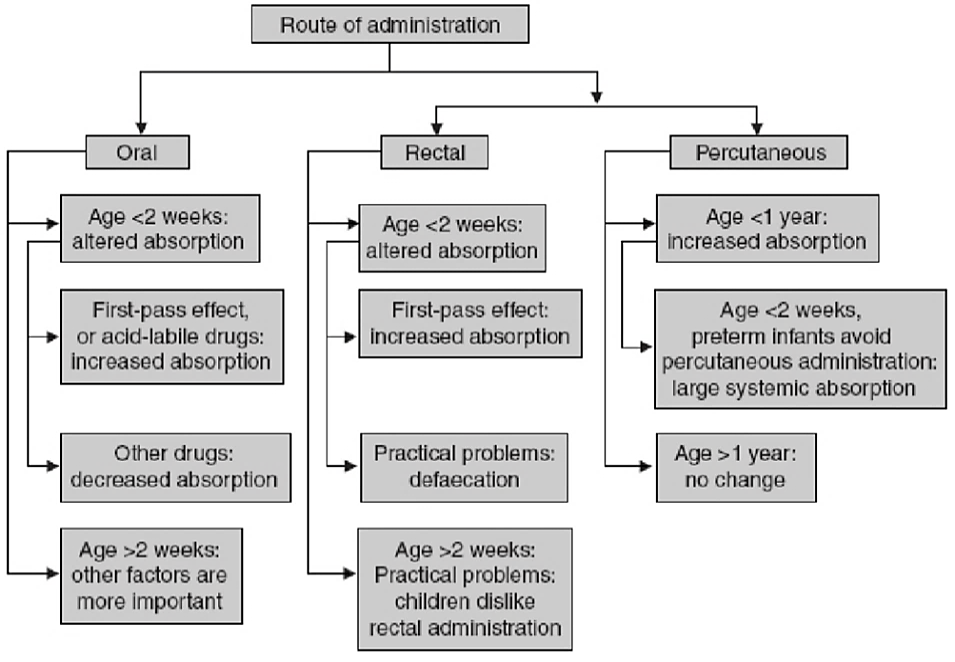
\includegraphics[width=.9\linewidth]{./pediatrie_administration.png}
\end{center}
\subsection{Posologies}
\label{sec:orge98b371}
\begin{itemize}
\item Posologie de l'enfant:
\[
  P_{enfant} = \frac{ S_{corporelle} \times D_{adulte} }{1.75}
  \]
\item Modifier selon les résultats biologiques:
\begin{itemize}
\item Fonctions rénales
\item Ionogramme sanguin
\end{itemize}
\item Par rapport aux indications:
\end{itemize}
\subsection{Erreurs d'Administration}
\label{sec:org2cacc96}
\begin{itemize}
\item IV: 48\% \emph{Facteur 10-100}
\item Formes buvables: Confusion \uline{mg/mL} et \uline{mg/kg}
\item Forme galénique non adaptée
\item Application cutanée: \textbf{passage systémique}
\end{itemize}
\subsection{Effets Indésirables}
\label{sec:org3dc627c}
\subsubsection{Croissance}
\label{sec:org2ca6dc2}
\begin{itemize}
\item Fluoroquinolones: contre-indiquées si < 8 ans \emph{sauf mucoviscidose}
\item Corticoïdes: ralentissement de la croissance
\item Tétracyclines: dischromie et hypoplasie dentaire
\end{itemize}
\subsubsection{Reye Syndrome}
\label{sec:org7ae5cb2}
\begin{itemize}
\item Associé à l'Aspirine si < 16 ans
\item Description: Atteinte cérébrale non-inflammatoire et hépatique
\end{itemize}
\subsubsection{Précautions et Contre-indications}
\label{sec:org64a705d}
\begin{itemize}
\item Acide benzoïque CI < 2 ans:
Risque d'ictère car fortement lié aux PP\footnote{Protéines plasmatiques}
\item Camphre: CI < 30 mois
Risque de convulsions
\item Acide borique et borate de Sodium \emph{(Talc, Cold Crean)}: CI < 3 ans
Risque de convulsions
\end{itemize}
\subsection{Formes Pharmaceutiques: Mésusage}
\label{sec:org84fa162}
\begin{center}
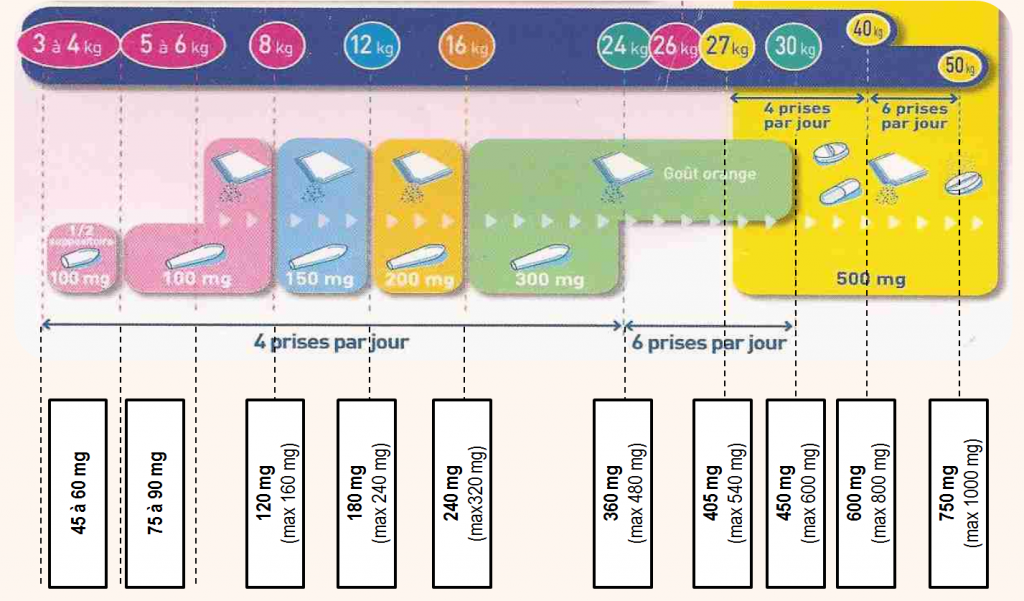
\includegraphics[width=.9\linewidth]{./pedia_galenique.png}
\end{center}
\subsubsection{Formes Orales Liquides}
\label{sec:orgb0911ab}
\begin{itemize}
\item Flacon multidose
\item Utilisation de présentation adulte
\item Instrument de mesure non adapté
\item Conservation
\item Absence de date d'ouverture
\item Prescription en unité différente de l'unité indiquée
\end{itemize}
\subsubsection{Formes Sèches}
\label{sec:orga7400a8}
\begin{itemize}
\item Prescription de demi ou quart de comprimé
\item Forme galénique inadaptée à l'âge
\item Déconditionnement de médicament
\begin{itemize}
\item Ouverture des gélules
\item Dispersion dans nourriture semi-solide
\item Dissolution dans un liquide
\item Broyage des comprimés
\item Fractionnement
\end{itemize}
\end{itemize}
\section{Analyse d'Ordonnance Pédiatrique}
\label{sec:orgdce5870}
\setlength{\parindent}{0pt}
\subsection{Prescription}
\label{sec:orgffa90c2}
\begin{itemize}
\item Date de la prescription
\item Identification du prescripteur
\item Signature
\item Identification du service
\item Identification du patient
\begin{itemize}
\item Nom
\item Prénom
\item Sexe
\item DDN\footnote{Date de naissance}
\item Pédiatrie:
\begin{itemize}
\item Poids
\end{itemize}
\item Si nécessaire:
\begin{itemize}
\item Taille
\item Surface corporelle
\end{itemize}
\end{itemize}
\item Identification du médicament
\begin{itemize}
\item DCI
\item Galénique
\item Dosage
\item Posologie
\item Administration
\item Mode d'emploi
\item Durée de traitement
\item Allergies
\end{itemize}
\end{itemize}
\subsection{Médicaments}
\label{sec:org3fa00f6}
\begin{itemize}
\item Indication précise
\item Bon choix
\item Posologie correcte
\begin{itemize}
\item Surtout si index thérapeutique étroit
\begin{itemize}
\item AVK
\item Acide Valproïque
\item Théophylline
\end{itemize}
\end{itemize}
\item Interactions
\begin{itemize}
\item Pharmacologiques
\item Physicochimiques
\end{itemize}
\item Modalités d'administration:
\begin{itemize}
\item Instruments de mesure
\item Pendant/En dehors des repas
\item Plans de prise
\item Conseils
\end{itemize}
\item Prescriptions hors-AMM
\end{itemize}
\subsection{Algorithme de Validation}
\label{sec:org589ae46}
\begin{figure}[htbp]
\centering
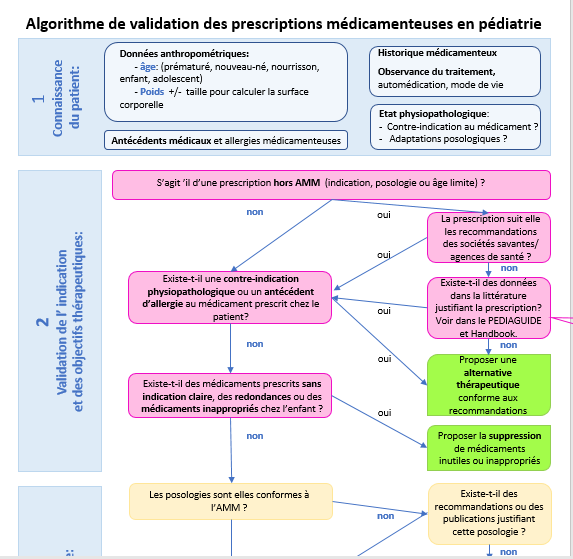
\includegraphics[width=.9\linewidth]{./pedia_validation2.png}
\caption{L'analyse se fait selon un algorithme de validation spécifique aux populations pédiatriques.}
\end{figure}
\subsection{Interactions Médicamenteuses}
\label{sec:org00658e5}
\begin{itemize}
\item Substances actives \(\Leftrightarrow\) substances auxilliaires
\item Molécules \(\Leftrightarrow\) test biologiques
\item Molécules \(\Leftrightarrow\) alimentation
\end{itemize}
\subsection{Rédiger un Plan de Prise}
\label{sec:org2fb2716}
\begin{center}
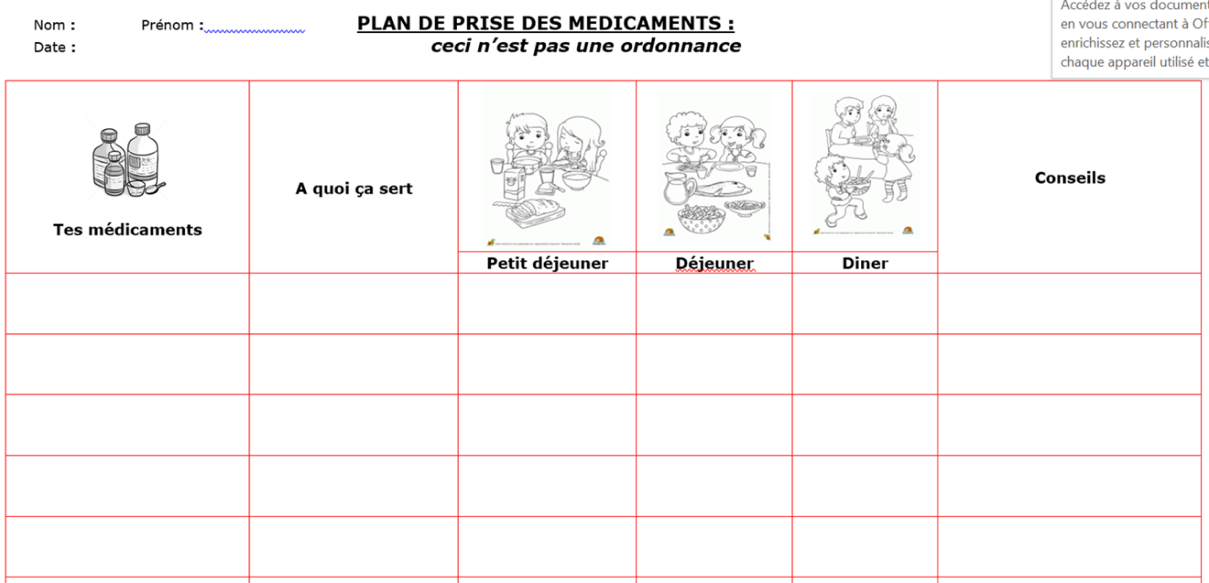
\includegraphics[width=.9\linewidth]{./plandeprise.png}
\end{center}
\section{Pharmacovigilance}
\label{sec:orgcabd6ee}
\setlength{\parindent}{0pt}
\subsection{Phase IV}
\label{sec:org18fd0ca}
La phase IV est la réévaluation de la sécurité et de l'efficacité d'un médicament après sa commercialisation.
\subsubsection{Objectifs}
\label{sec:org8f503bc}
\begin{itemize}
\item Recenser les EI \footnote{Effets indésirables}
\item Identifier les IAM \footnote{Intéractions médicamenteuses}
\item Evaluer et quantifier sur de grandes populations, en situation réelle, l'efficacité et la tolérance des médicaments.
\item Vérifier et modifier si nécessaire les indications du médicament.
\end{itemize}
\subsection{Pharmacovigilance}
\label{sec:org556a094}
\subsubsection{Médicaments Concernés}
\label{sec:org41b1e98}
\begin{itemize}
\item AMM
\item ATU
\item MDS
\item Homéopatie
\end{itemize}
\subsubsection{A Qui Déclarer?}
\label{sec:orgb146897}
\begin{itemize}
\item CRPV \footnote{Centre Régional de Pharmacovigilance}
\item Industrie pharmaceutique (facultative)
\end{itemize}
\begin{center}
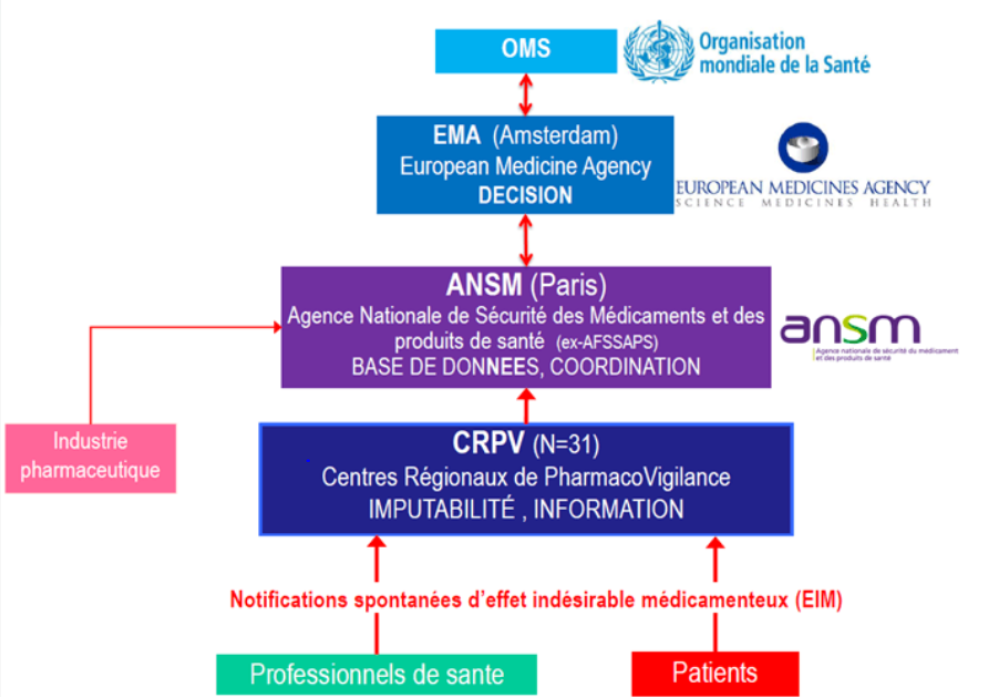
\includegraphics[width=.9\linewidth]{./crpv.png}
\end{center}
\subsubsection{Evalutation des Notifications}
\label{sec:org6d77f33}
\begin{enumerate}
\item Imputabilités
\label{sec:org509e655}
\begin{center}
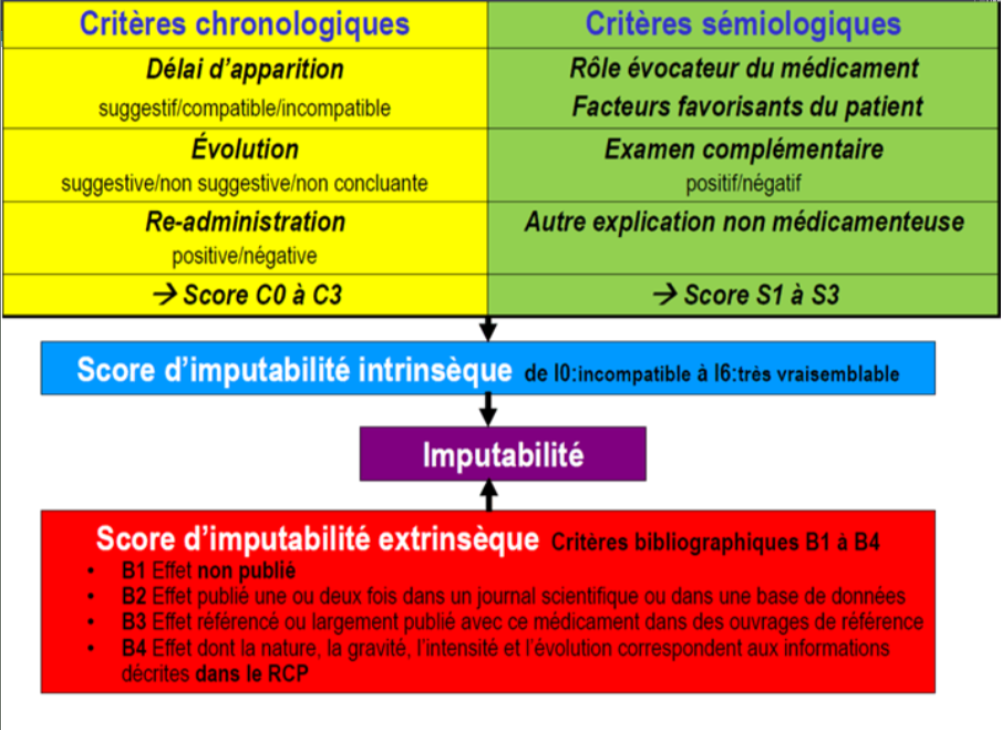
\includegraphics[width=.9\linewidth]{./imputabilite.png}
\end{center}
\begin{enumerate}
\item Intrinsèque
\label{sec:orgef5801e}
\begin{itemize}
\item critère chronologique
\item critère sémiologique
\end{itemize}
\item Extrinsèque
\label{sec:org38a4ede}
\begin{itemize}
\item critère bibliographique
\end{itemize}
\end{enumerate}
\end{enumerate}
\section{Médicaments à Statut Particulier}
\label{sec:org6f00486}
\setlength{\parindent}{0pt}

\subsection{Stupéfiants}
\label{sec:org73183aa}
Une prescription de stupéfiant doit contenir la dose et la posologie.
Le patient à \textbf{72 heures} pour recevoir une dispensation complète de son traitement\footnote{Sinon il faudra déconditionner}.

Le pharmacien doit les stocker dans une armoire \textbf{fermée à clef différente} de celle des stupéfiants détenus à l'officine

Le transport à l'étranger pour un patient doit se faire par une \textbf{autorisation de transport de l'ARS locale au médecin prescripteur}.

La morphine injectable peut être prescripte pour \textbf{7 jours} maximum.

La délivrance de FENTANYL \emph{adm: patch, buccale, ou nasale} pour les douleurs chroniques doit être fractionnée \textbf{sauf mention expresse du prescripteur}

La Méthadone peut être prescrite jusqu'à \textbf{28 jours}, et délivrée par fractions de \textbf{7 jours} sauf mention expresse du prescripteur.

\subsubsection{Ordonnance}
\label{sec:org422a202}
\begin{itemize}
\item Sécurisée
\item Doit afficher \emph{en toutes lettres}:
\begin{itemize}
\item le nombre d'unité par prise
\item Nombre de prise
\item dosage
\end{itemize}
\end{itemize}

\begin{center}
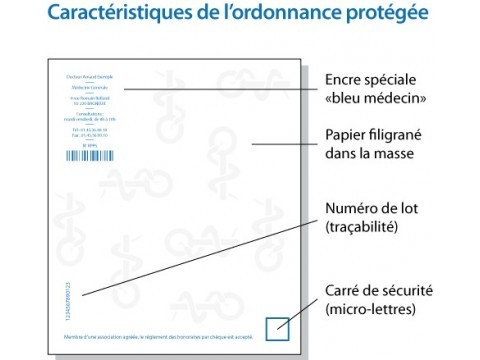
\includegraphics[width=.9\linewidth]{./ordo_securisee.png}
\end{center}

\subsubsection{Délivrance}
\label{sec:org1da8338}
\begin{center}
\begin{tabular}{lll}
DCI & Fractionnement & Exemples\\
\hline
Fentanyl \emph{transdermique} & 14 j & Durogesic, Matrifen\\
Fentanyl \emph{transmuqueuse} & 7 j & Actiq, Effentora, Abstral, Instanyl, Pecfent\\
Methadone & 7 j & \\
\end{tabular}
\end{center}

\subsubsection{Mentions à Apposer}
\label{sec:orga8f2701}
\begin{itemize}
\item Tampon de l'officine
\item N° enregistrement sur l'ordonnancier
\item Date de délivrance
\item Nom de la spécialité délivrée
\item Quantité délivrée en unité de prise
\end{itemize}

\subsubsection{Comptabilité et Traçabilité}
\label{sec:orgc193b64}
\begin{itemize}
\item Comptabilité journalière
\item Balance mensuelle
\item Inventaire annuel du stock
\item Conservation des ordonnances pendant 10 ans
\end{itemize}

\subsection{Assimilés Stupéfiants}
\label{sec:org881da0c}
Ils sont prescrits sur une ordonnance sécurisée, et sont stockés dans un lieu avec accès restreint.
Le patient à 3 mois pour reçevoir la totalité de sa prescription\footnote{Pas de déconditionnement possible.}.

La durée de prescription maximale dépend du médicament, fixée par arrêté ministériel.

Tous les AS \footnote{Assimilé stupéfiant} ne sont pas renouvellables.

\subsection{Anxiolytiques et Hypnotiques}
\label{sec:orge028f5e}

\subsubsection{Première délivrance}
\label{sec:org04fb687}
Elle se fait uniquement sur une ordonnance datant de moins de 3 mois.

\subsubsection{Prescription et Règles de Délivrance}
\label{sec:org6b3ba0c}
\begin{center}
\begin{tabular}{ll}
Hypnotiques & 4 semaines\\
Anxiolytiques & 12 semaines\\
\end{tabular}
\end{center}

\emph{Il est interdit de renouveller de manière exceptionnelle un anxiolytique ou hypnotique}

\subsection{Médicaments d'Exception}
\label{sec:org8e18c4f}
Ce sont des spécialités remboursées uniquement pour certaines indications.
Leur prescription se fait alors sur une ordonnance 4 volets\footnote{Conforme au Cerfa 12708*02}.

\begin{center}
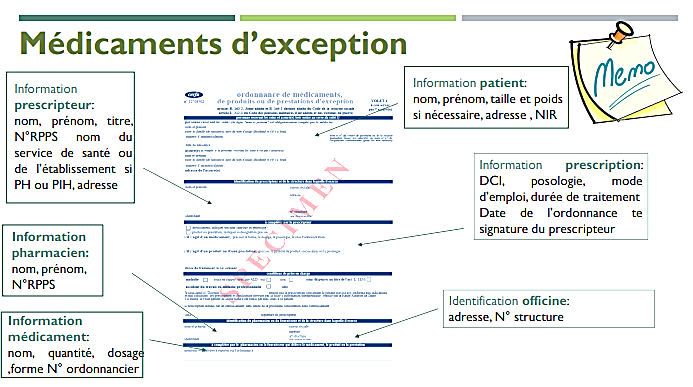
\includegraphics[width=.9\linewidth]{./exception.png}
\end{center}

\subsubsection{Mentions à Apposer}
\label{sec:orga2de9b8}
\begin{itemize}
\item Tampon de l'officine
\item N° RPPS du dispensateur
\item Date de délivrance
\item Nom de la spécialité délivrée
\item Quantité délivrée en unité de prise
\end{itemize}


\subsubsection{Archivage}
\label{sec:orga04c9b8}
\begin{itemize}
\item Volet 4 archivé par le pharmacien
\item Durée de conservation de 3 ans.
\end{itemize}

\subsection{Prescription Compassionnelle}
\label{sec:org723f4af}
Un CPC\footnote{Prescription Compassionnelle} peut être mis en place pour une durée maximale de 3 ans.
La spécialité sela alors prise en charge par la sécurité sociale.

Le CPC permet d'encadrer de manière ponctuelle l'utilisation d'un médicament \textbf{hors AMM}.
Au regard des données recueillies, le CPC peut conduire à autoriser la modification de l'AMM du médicament.

\subsection{Prescription Hospitalière}
\label{sec:orgd43c514}

\subsubsection{Prescription Initiale Hospitalière}
\label{sec:org9db7f66}
La dispensation se fait sur présentation \textbf{concomitante} de l'ordonnance hospitalière initiale.
Le renouvellement se fait par tout prescripteur \textbf{sauf restriction particulières (spécialistes)}

\subsubsection{Prescription Réservée à Certains Spécialites}
\label{sec:org1dee536}
Il est important de s'assurer de l'habilitation du prescripteur.

\subsection{Médicaments Nécessitant une Surveillance Particulière}
\label{sec:orgbb425ef}
Les restrictions sont dues aux potentiels effets indésirables graves qui peuvent apparaître lors de l'emploi de la spécialité.

\subsubsection{Condition de Prescription}
\label{sec:org0be6593}
Subordonnée à la réalisation d'examens périodiques du patient.
La mise à disposition d'un support d'information/de suivi de traitement peut être \emph{imposée} lors de la mise sur le marché du médicament.

\subsubsection{Conditions de Délivrance}
\label{sec:org7281bd6}
Le pharmacien doit s'assurer l'habilitation du prescripteur à prescrire le produit, ou le cas échéant de la présence sur l'ordonnance des mentions obligatoires prévues par l'AMM.

\subsection{Médicaments Dérivés du Sang}
\label{sec:org6fc6f6f}
Prescription: ordonnance classique

La dispensation d'un MDS est retranscrite dans un registre paraphé par le maire ou le commissaire de police.

\subsubsection{Traçabilité}
\label{sec:orgd9bfe60}
Les informations suivantes doivent figurer sur le registre spécial :
\begin{itemize}
\item Nom et adresse du prescripteur
\item Nom, adresse et date de naissance du patient
\item Date de délivrance
\item Dénomination du médicament
\item Quantité délivrée
\item Les informations figurant sur l'étiquette de traçabilité détachable du conditionnement
\end{itemize}
extérieur

\subsection{Médicaments à Usage Professionnel}
\label{sec:org60f8e13}
L'AMM peut prévoir la délivrance d'un produit qu'à des professionnels de santé habilités à la prescrire et à l'administrer. Cette sécurité est liée à la nécessité d'une détention et d'une manipulation exclusive par un professionnel de santé.

\subsubsection{Ordonnance}
\label{sec:orgba079a4}
\begin{itemize}
\item Nom
\item Qualité
\item RPPS
\item Adresse
\item Date

En plus,
\item Dénomination
\item Quantité
\item Mention: "Usage Professionnel"
\end{itemize}
\section{Compétences et Responsabilités du Pharmacien}
\label{sec:orgb8c9648}
\setlength{\parindent}{0pt}
\subsection{L'Ordre National des Pharmaciens}
\label{sec:org79f30af}

\begin{center}
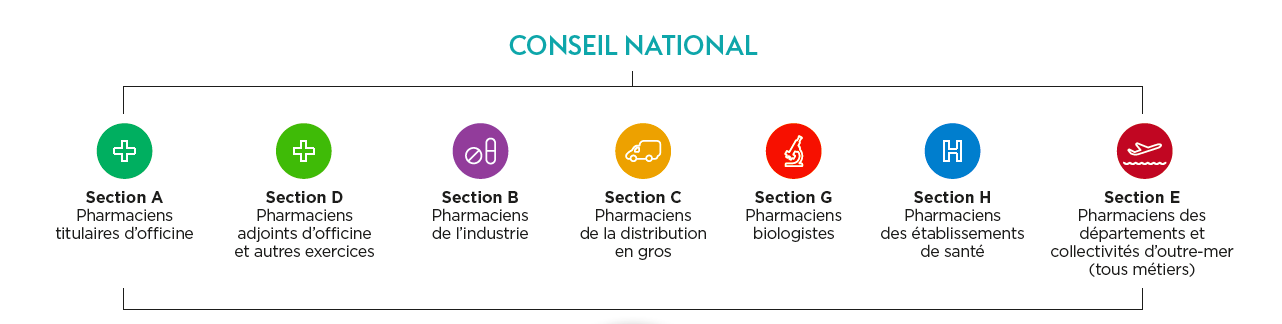
\includegraphics[width=.9\linewidth]{./ordre.png}
\end{center}
\subsubsection{Missions}
\label{sec:org5577469}
\begin{itemize}
\item Garantir le respect des devoirs professionnels
\item Protéger l'intégrité et l'indépendance de la profession
\item Garantir la compétence des pharmaciens
\item Contribuer à promouvoir la santé publique, la qualité des soins notamment la sécurité des actes professionnels.
\item S'assurer que l'ensemble des pharmaciens respecte son obligation de développement professionnel continu
\end{itemize}
\end{document}